\documentclass[12pt,a4paper]{article}

% --- Packages ---
\usepackage[margin=1in]{geometry}
\usepackage{graphicx}
\usepackage{titling}
\usepackage{fancyhdr}
\usepackage{hyperref}
\usepackage{xcolor}
\usepackage{float}

% --- Page Style ---
\pagestyle{fancy}
\fancyhf{}
\fancyhead[L]{\small Module 5 -- JDBC Assignment}
\fancyhead[R]{\small Mausam Kar | 24BAI10284}
\fancyfoot[C]{\thepage}
\renewcommand{\headrulewidth}{0.4pt}
\renewcommand{\footrulewidth}{0.4pt}

% --- Title ---
\title{%
  \vspace{-1cm}
  \textbf{\Large Module 5: JDBC Programming Assignment}\\[6pt]
  \large Connect a Database Using JDBC Driver ---\\
  Submitting Queries and Getting Results from the Database
}
\author{%
  \textbf{Mausam Kar}\\
  Registration No: \textbf{24BAI10284}
}
\date{\today}

\begin{document}

% --- Title Page ---
\maketitle
\thispagestyle{fancy}

\vspace{0.5cm}

\section*{Objective}
Write a Java program to connect a database by using a JDBC driver --- submitting queries and getting results from the database. The program demonstrates all CRUD (Create, Read, Update, Delete) operations along with aggregate queries using JDBC with an SQLite embedded database.

\vspace{0.3cm}
\noindent\textbf{Technologies Used:}
\begin{itemize}
  \item Java (JDK 21+)
  \item JDBC API (\texttt{java.sql.*})
  \item SQLite Database (embedded, via \texttt{sqlite-jdbc} driver)
\end{itemize}

\newpage

% -------------------------------------------------------
% CODE SCREENSHOTS
% -------------------------------------------------------
\section{Program Code}

The complete Java source code for the JDBC database operations program is shown below across multiple screenshots.

\vspace{0.3cm}

\begin{figure}[H]
  \centering
  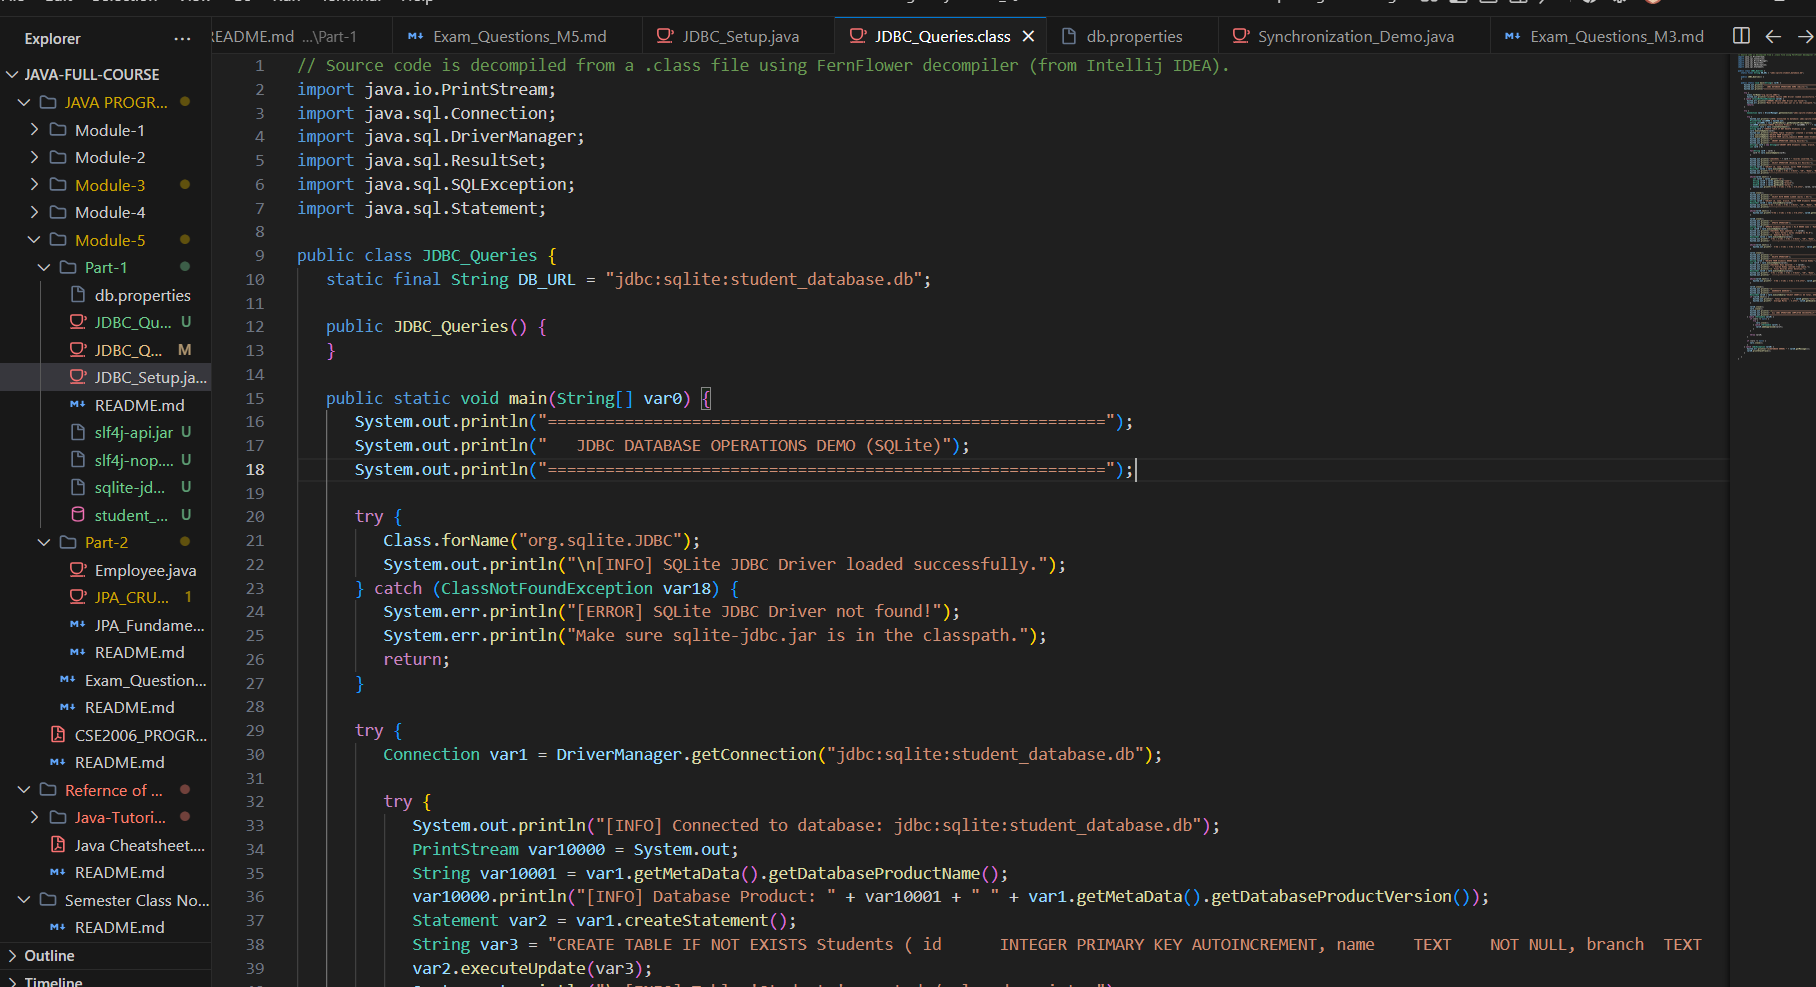
\includegraphics[width=\textwidth]{Code1.png}
  \caption{Code Part 1 -- Imports, class declaration, driver loading, and connection setup}
\end{figure}

\begin{figure}[H]
  \centering
  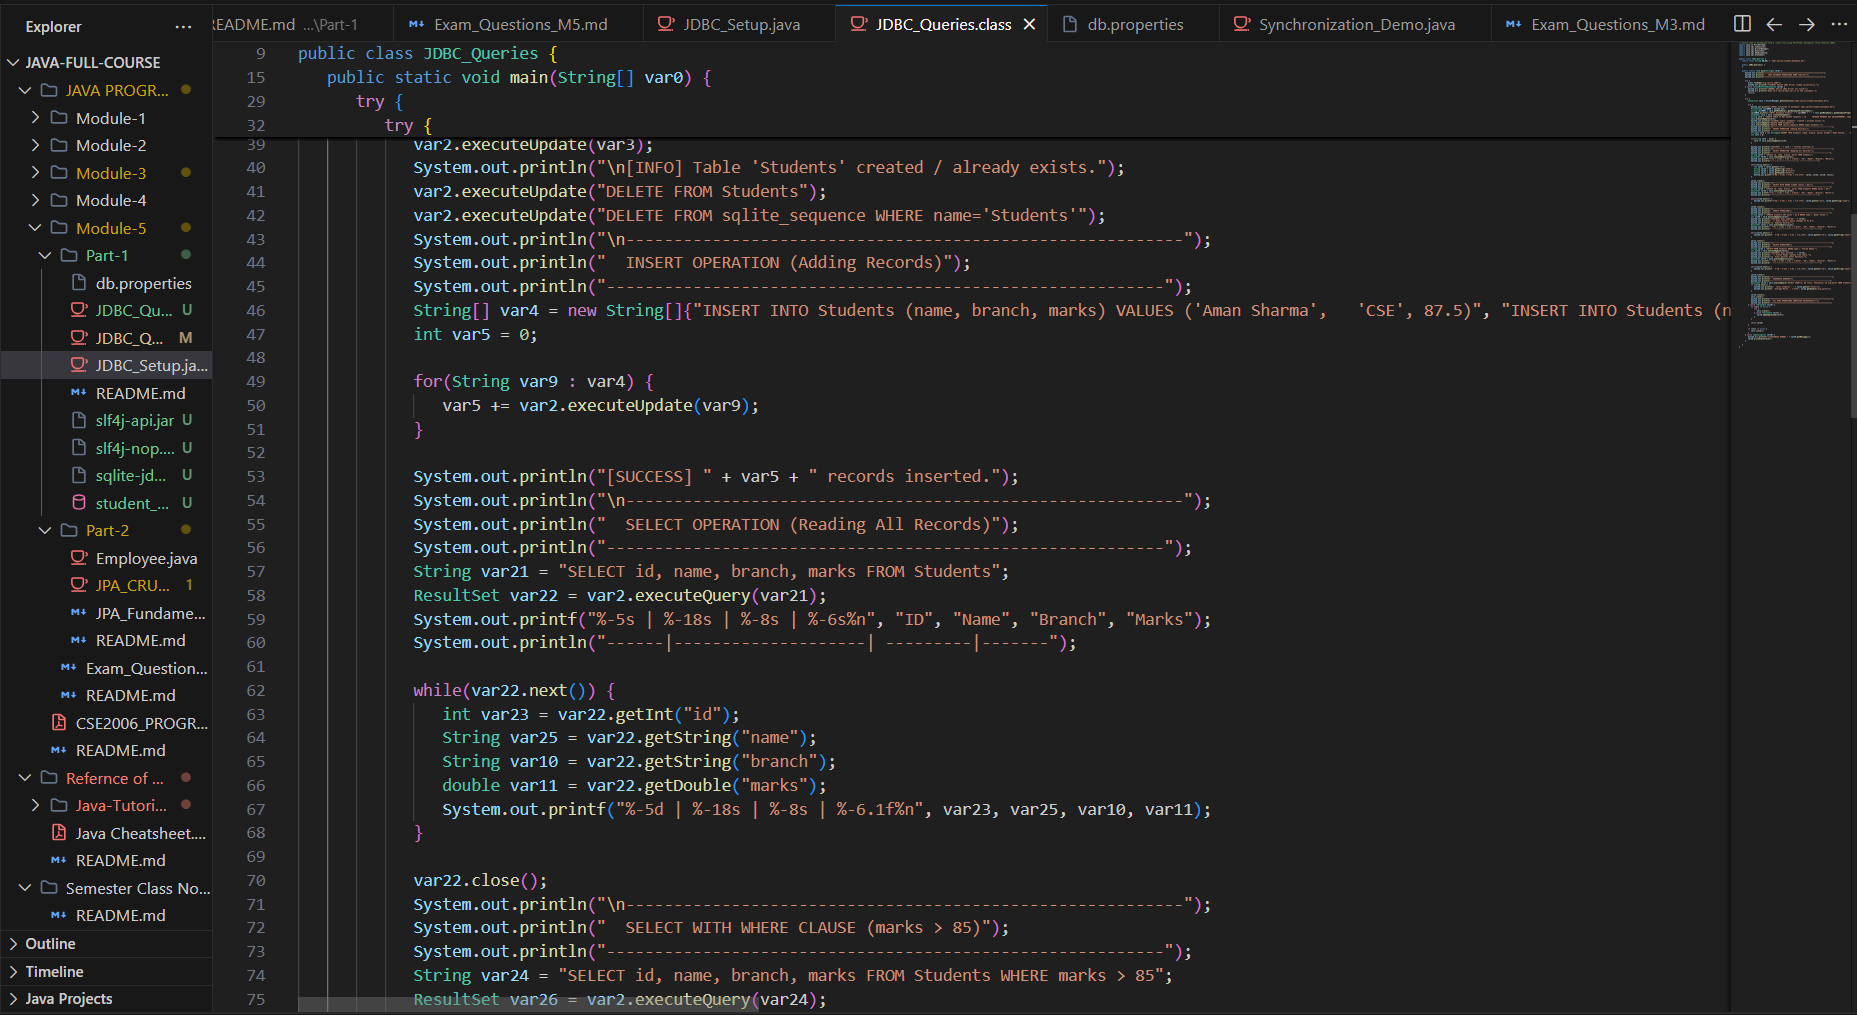
\includegraphics[width=\textwidth]{code2.png}
  \caption{Code Part 2 -- CREATE TABLE and INSERT operations}
\end{figure}

\begin{figure}[H]
  \centering
  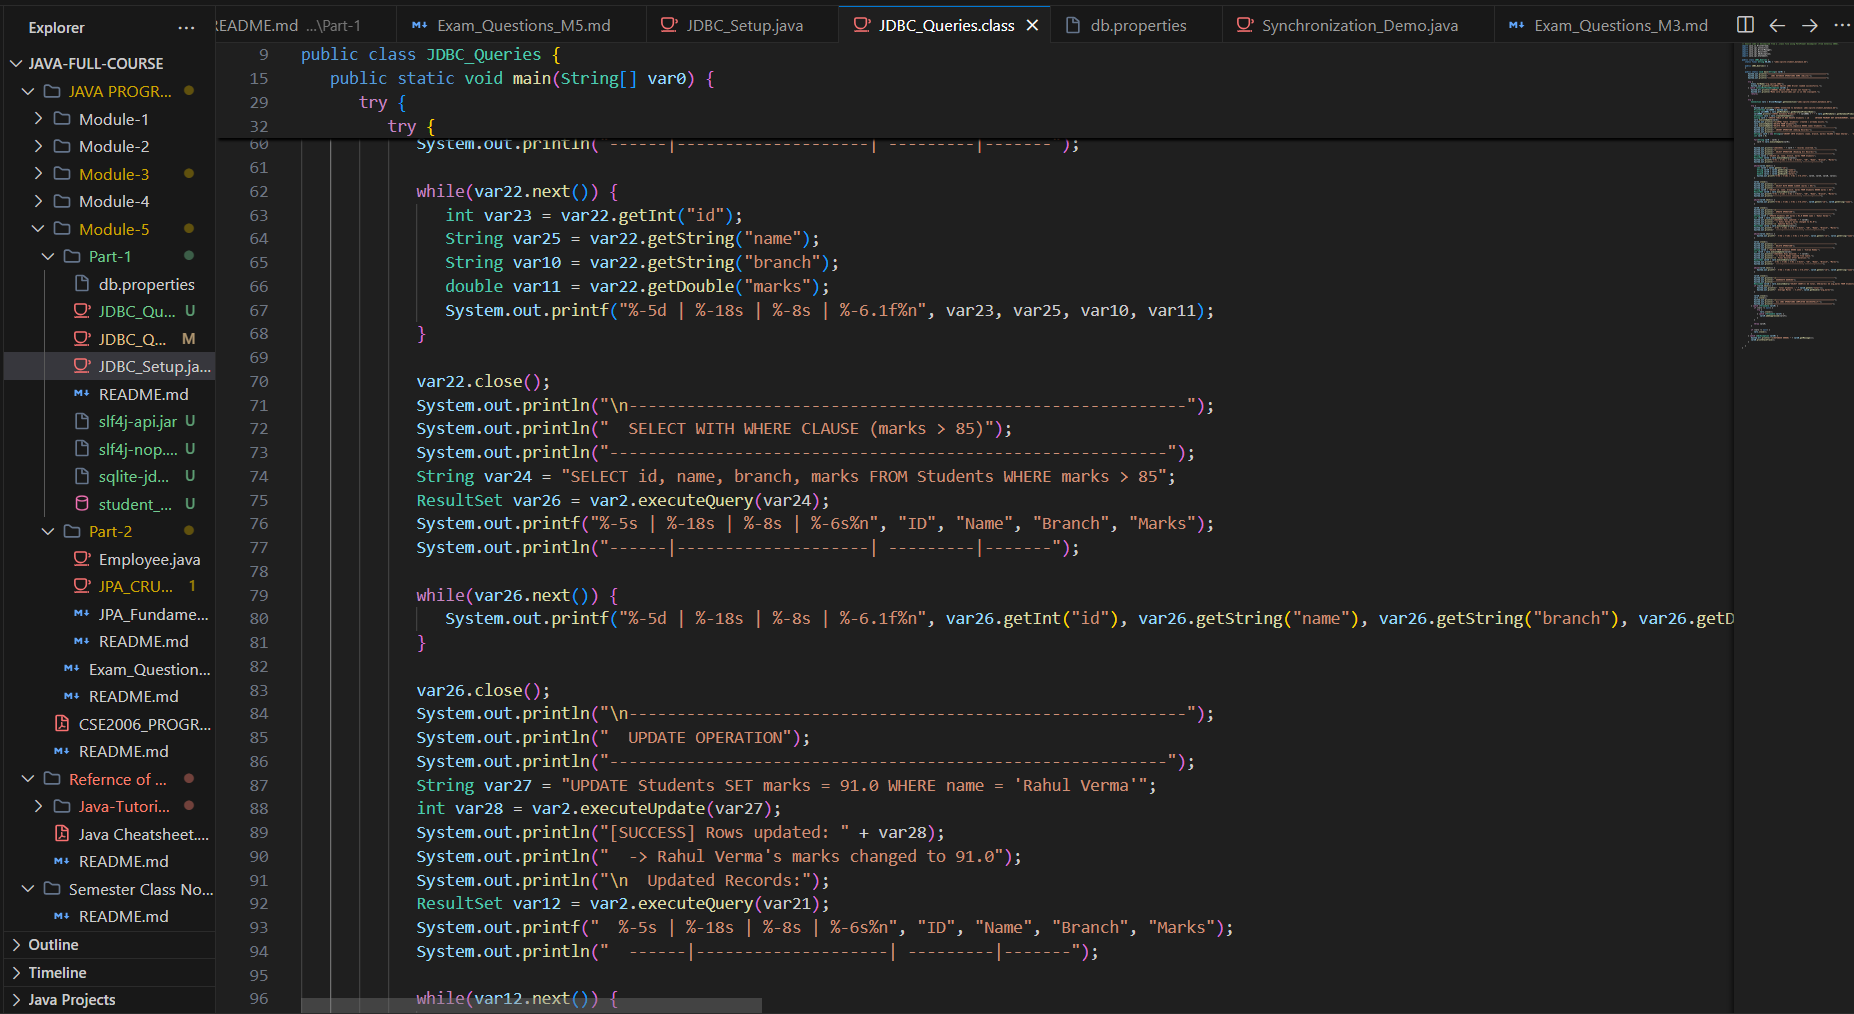
\includegraphics[width=\textwidth]{Code3.png}
  \caption{Code Part 3 -- SELECT query with ResultSet traversal}
\end{figure}

\begin{figure}[H]
  \centering
  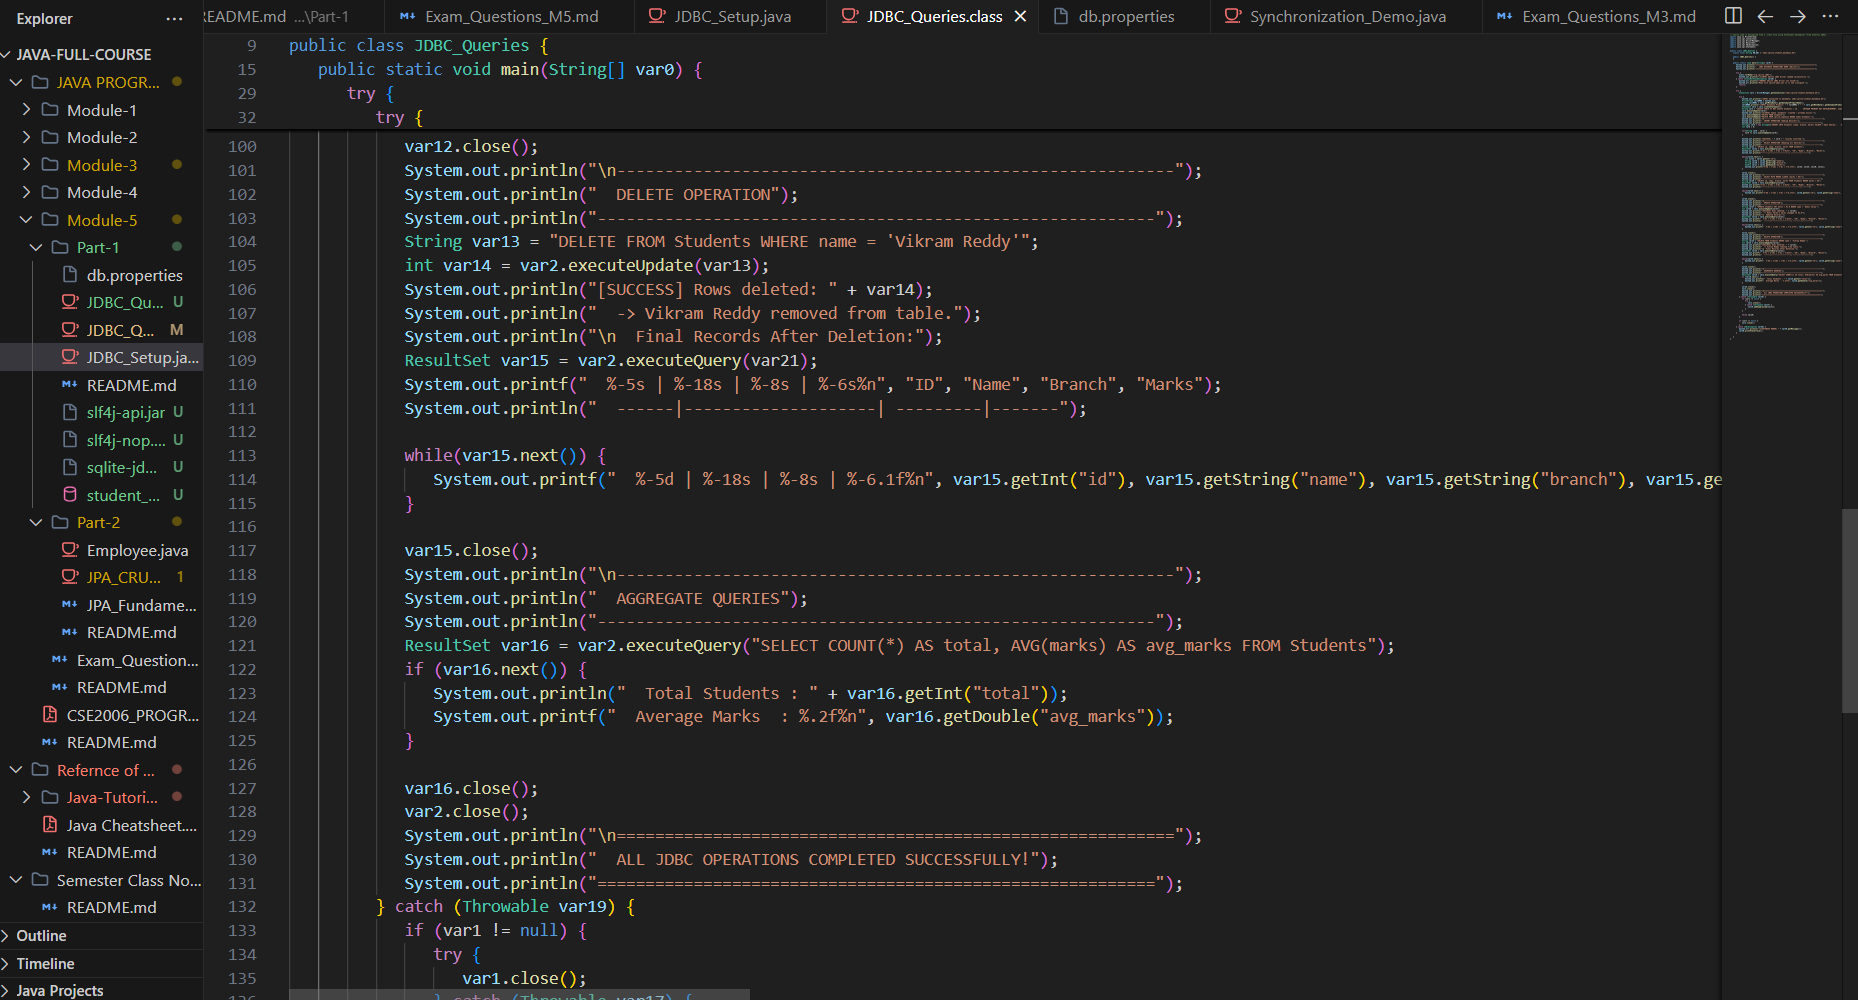
\includegraphics[width=\textwidth]{Code4.png}
  \caption{Code Part 4 -- UPDATE and DELETE operations with result display}
\end{figure}

\begin{figure}[H]
  \centering
  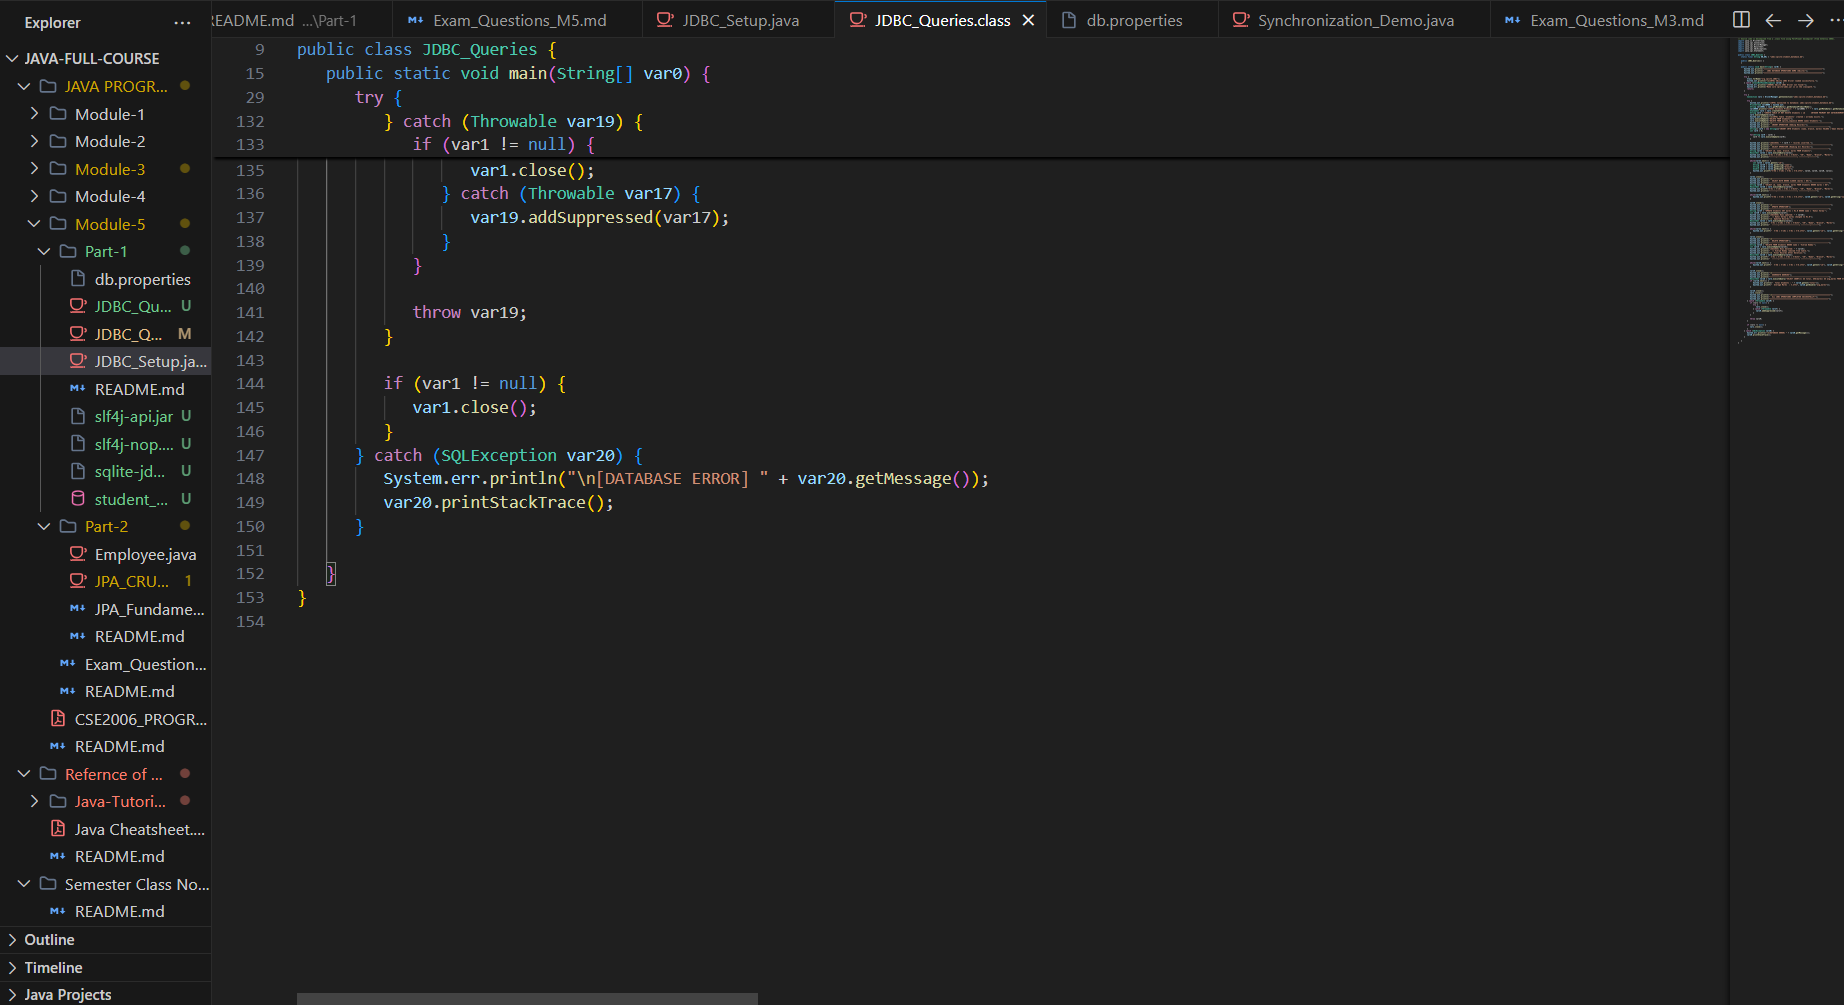
\includegraphics[width=\textwidth]{Code5.png}
  \caption{Code Part 5 -- Aggregate queries (COUNT, AVG) and closing}
\end{figure}

\newpage

% -------------------------------------------------------
% OUTPUT SCREENSHOTS
% -------------------------------------------------------
\section{Program Output}

The program was compiled and executed successfully. The output screenshots are shown below.

\vspace{0.2cm}
\noindent\textbf{Commands used:}
\begin{verbatim}
javac -cp ".;sqlite-jdbc.jar" JDBC_Queries.java
java -cp ".;sqlite-jdbc.jar;slf4j-api.jar;slf4j-nop.jar" JDBC_Queries
\end{verbatim}

\begin{figure}[H]
  \centering
  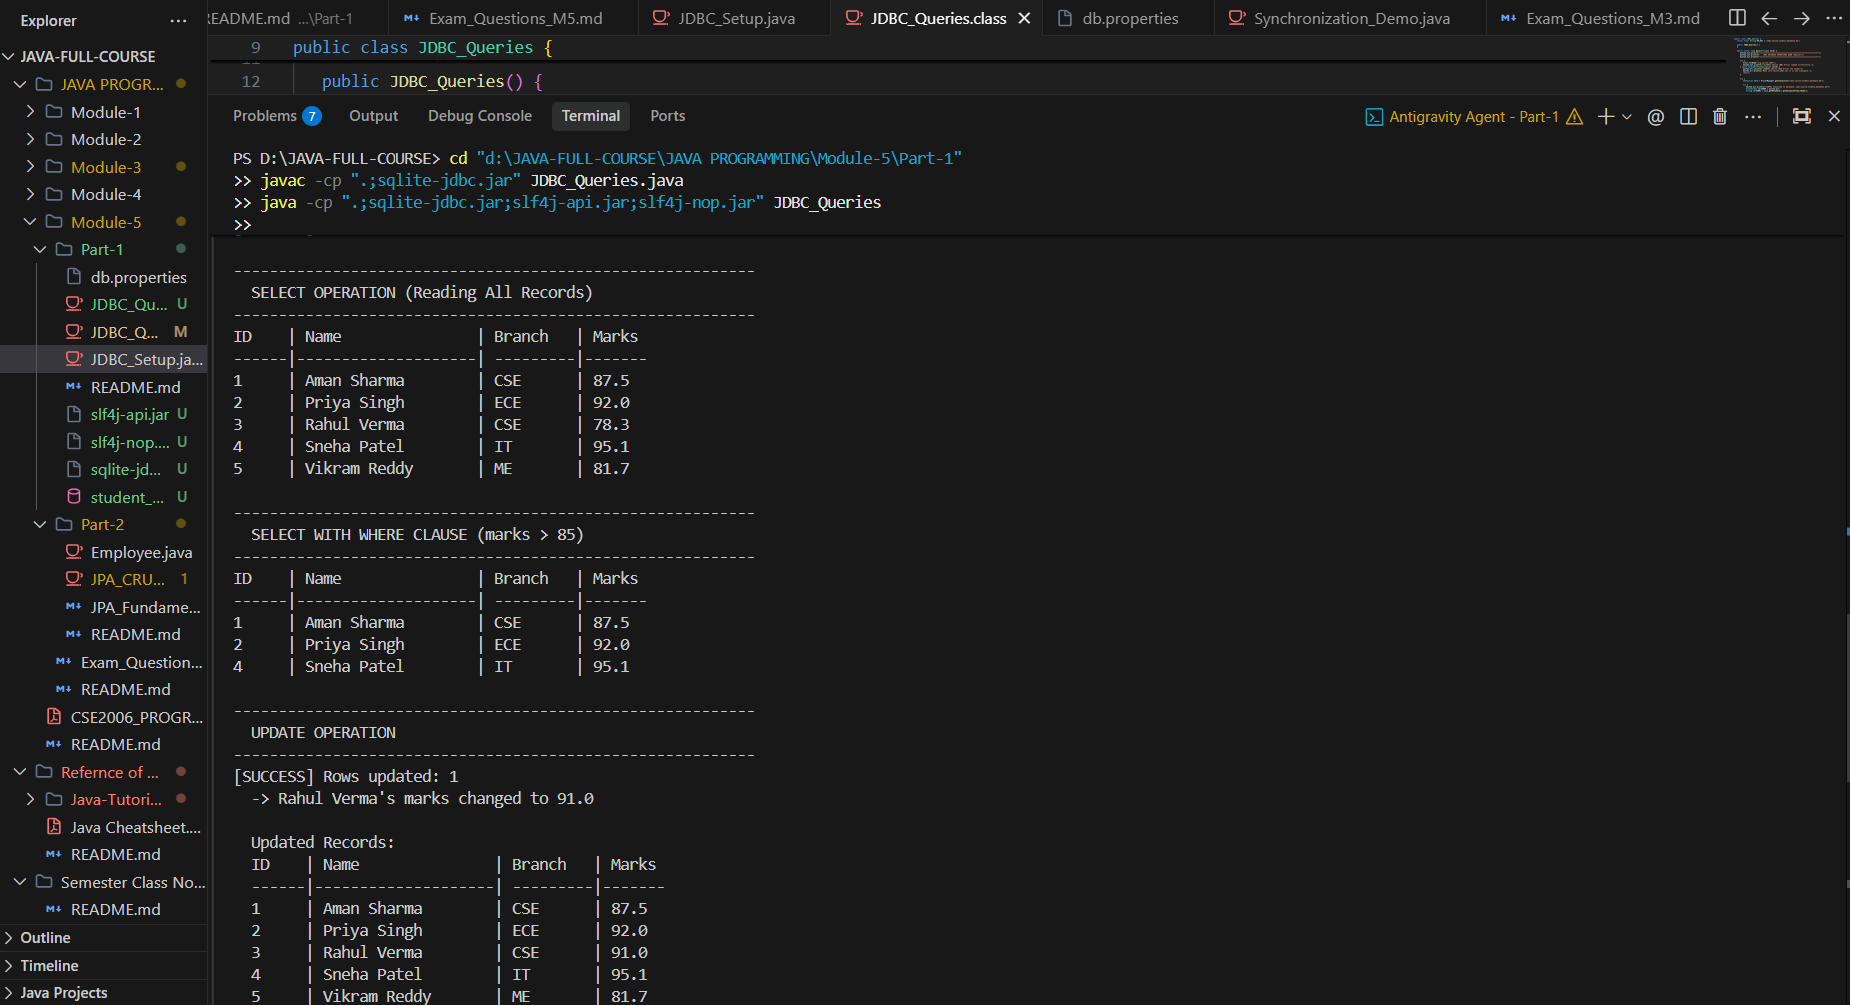
\includegraphics[width=\textwidth]{Output1.png}
  \caption{Output Part 1 -- Connection, INSERT, SELECT all records, and filtered SELECT}
\end{figure}

\begin{figure}[H]
  \centering
  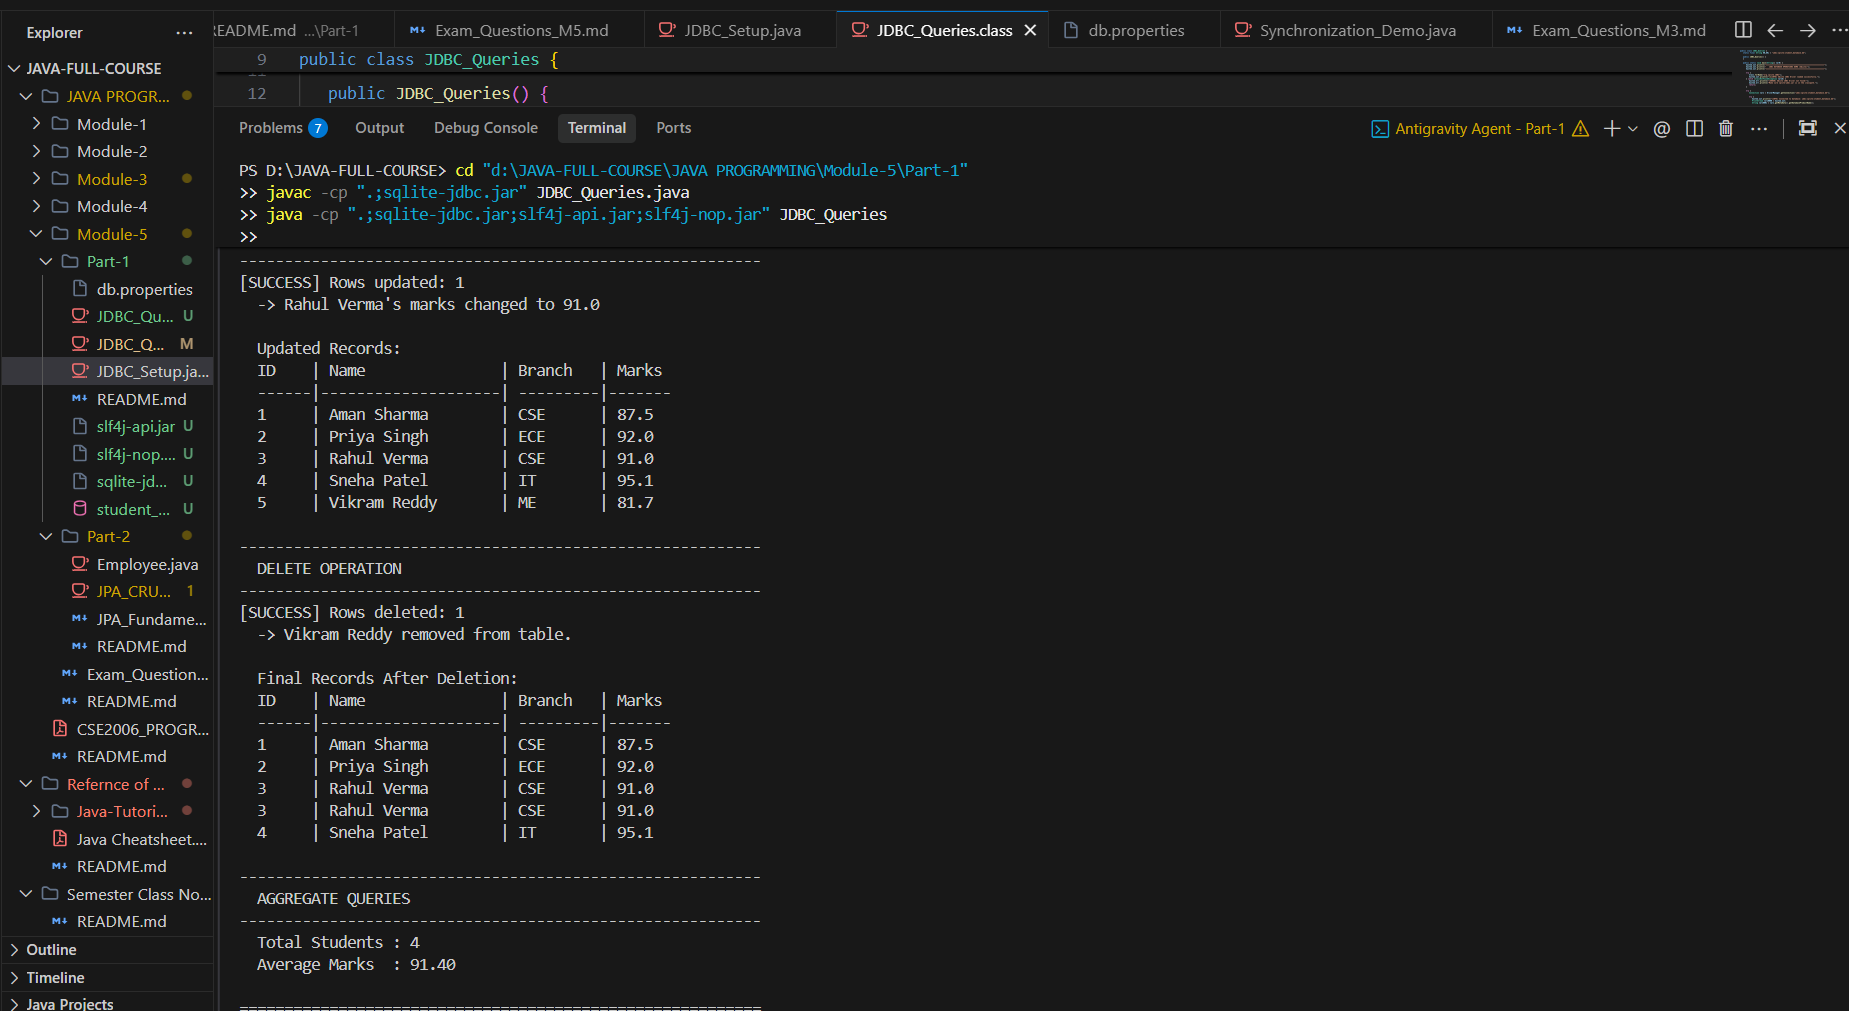
\includegraphics[width=\textwidth]{Output2.png}
  \caption{Output Part 2 -- UPDATE, DELETE results, and aggregate queries}
\end{figure}

\newpage

% -------------------------------------------------------
% CONCLUSION
% -------------------------------------------------------
\section{Conclusion}

The program successfully demonstrates:
\begin{enumerate}
  \item \textbf{JDBC Driver Loading} -- Using \texttt{Class.forName()} to load the SQLite JDBC driver.
  \item \textbf{Database Connection} -- Establishing connection via \texttt{DriverManager.getConnection()}.
  \item \textbf{CREATE TABLE} -- Creating the \texttt{Students} table with appropriate schema.
  \item \textbf{INSERT (Create)} -- Adding 5 student records into the database.
  \item \textbf{SELECT (Read)} -- Querying all records and filtering with \texttt{WHERE} clause using \texttt{ResultSet}.
  \item \textbf{UPDATE} -- Modifying existing records (\texttt{Rahul Verma's marks updated to 91.0}).
  \item \textbf{DELETE} -- Removing a record (\texttt{Vikram Reddy} removed from the table).
  \item \textbf{Aggregate Queries} -- Computing \texttt{COUNT(*)} and \texttt{AVG(marks)}.
  \item \textbf{Resource Management} -- Using \texttt{try-with-resources} for automatic connection cleanup.
\end{enumerate}

\vspace{1cm}
\noindent\rule{\textwidth}{0.4pt}
\begin{center}
  \textbf{Submitted by:} Mausam Kar \quad|\quad \textbf{Reg. No:} 24BAI10284
\end{center}

\end{document}
